\documentclass[11pt]{article}
\usepackage[margin=0.7in]{geometry}
\usepackage{graphicx}
\usepackage{booktabs}
\usepackage{float}
\begin{document}
\title{Data Mining Assignment 4: Classification Readme}
\author{}
\date{}
\maketitle
\section*{Datasets and Preprocessing}
All datasets were split in an 80/20 stratified ratio. Missing values were imputed inside the training pipeline. Numeric outliers were clipped using the 1.5 IQR rule before modeling.
\begin{tabular}{lrrrrl}
\toprule
      dataset &   rows &  features &  train\_rows &  test\_rows &                        classes \\
\midrule
     cervical &    858 &        28 &         686 &        172 &                Cancer, Healthy \\
 fetal\_health &   2126 &        21 &        1700 &        426 &  Normal, Pathological, Suspect \\
      banking &  41188 &        20 &       32950 &       8238 &                        No, Yes \\
\bottomrule
\end{tabular}

\section*{5-Fold Cross-Validation Mean Metrics}
\begin{tabular}{lllrrrrr}
\toprule
      dataset &          model &                 backend &  precision\_weighted &  recall\_weighted &  f1\_weighted &  accuracy &  auc\_roc \\
\midrule
      banking &       AdaBoost &      AdaBoostClassifier &              0.9037 &           0.9111 &       0.9063 &    0.9111 &   0.9421 \\
      banking &  Decision Tree &  DecisionTreeClassifier &              0.9049 &           0.8801 &       0.8895 &    0.8801 &   0.8059 \\
      banking &  Random Forest &  RandomForestClassifier &              0.9183 &           0.9069 &       0.9114 &    0.9069 &   0.9433 \\
      banking &        XGBoost &           XGBClassifier &              0.9014 &           0.9122 &       0.9026 &    0.9122 &   0.9444 \\
     cervical &       AdaBoost &      AdaBoostClassifier &              0.8892 &           0.9038 &       0.8955 &    0.9038 &   0.4859 \\
     cervical &  Decision Tree &  DecisionTreeClassifier &              0.8872 &           0.8309 &       0.8566 &    0.8309 &   0.5371 \\
     cervical &  Random Forest &  RandomForestClassifier &              0.8906 &           0.9227 &       0.9053 &    0.9227 &   0.5985 \\
     cervical &        XGBoost &           XGBClassifier &              0.8813 &           0.9329 &       0.9055 &    0.9329 &   0.6141 \\
 fetal\_health &       AdaBoost &      AdaBoostClassifier &              0.9148 &           0.9106 &       0.9112 &    0.9106 &   0.9521 \\
 fetal\_health &  Decision Tree &  DecisionTreeClassifier &              0.9061 &           0.8894 &       0.8944 &    0.8894 &   0.9196 \\
 fetal\_health &  Random Forest &  RandomForestClassifier &              0.9254 &           0.9259 &       0.9252 &    0.9259 &   0.9824 \\
 fetal\_health &        XGBoost &           XGBClassifier &              0.9258 &           0.9276 &       0.9256 &    0.9276 &   0.9823 \\
\bottomrule
\end{tabular}

\section*{Held-Out Test Metrics}
\begin{tabular}{lllrrrrr}
\toprule
      dataset &          model &                 backend &  precision\_weighted &  recall\_weighted &  f1\_weighted &  accuracy &  auc\_roc \\
\midrule
     cervical &  Decision Tree &  DecisionTreeClassifier &              0.8915 &           0.8140 &       0.8483 &    0.8140 &   0.5536 \\
     cervical &  Random Forest &  RandomForestClassifier &              0.9020 &           0.9302 &       0.9111 &    0.9302 &   0.5641 \\
     cervical &        XGBoost &           XGBClassifier &              0.8758 &           0.9302 &       0.9022 &    0.9302 &   0.5776 \\
     cervical &       AdaBoost &      AdaBoostClassifier &              0.8748 &           0.9128 &       0.8934 &    0.9128 &   0.5127 \\
 fetal\_health &  Decision Tree &  DecisionTreeClassifier &              0.9143 &           0.9014 &       0.9055 &    0.9014 &   0.9327 \\
 fetal\_health &  Random Forest &  RandomForestClassifier &              0.9355 &           0.9343 &       0.9348 &    0.9343 &   0.9835 \\
 fetal\_health &        XGBoost &           XGBClassifier &              0.9442 &           0.9460 &       0.9444 &    0.9460 &   0.9799 \\
 fetal\_health &       AdaBoost &      AdaBoostClassifier &              0.9073 &           0.8967 &       0.9004 &    0.8967 &   0.9434 \\
      banking &  Decision Tree &  DecisionTreeClassifier &              0.9034 &           0.8813 &       0.8898 &    0.8813 &   0.7989 \\
      banking &  Random Forest &  RandomForestClassifier &              0.9197 &           0.9087 &       0.9131 &    0.9087 &   0.9444 \\
      banking &        XGBoost &           XGBClassifier &              0.9043 &           0.9145 &       0.9051 &    0.9145 &   0.9471 \\
      banking &       AdaBoost &      AdaBoostClassifier &              0.9037 &           0.9116 &       0.9063 &    0.9116 &   0.9460 \\
\bottomrule
\end{tabular}

\section*{Figures}
\begin{figure}[H]\centering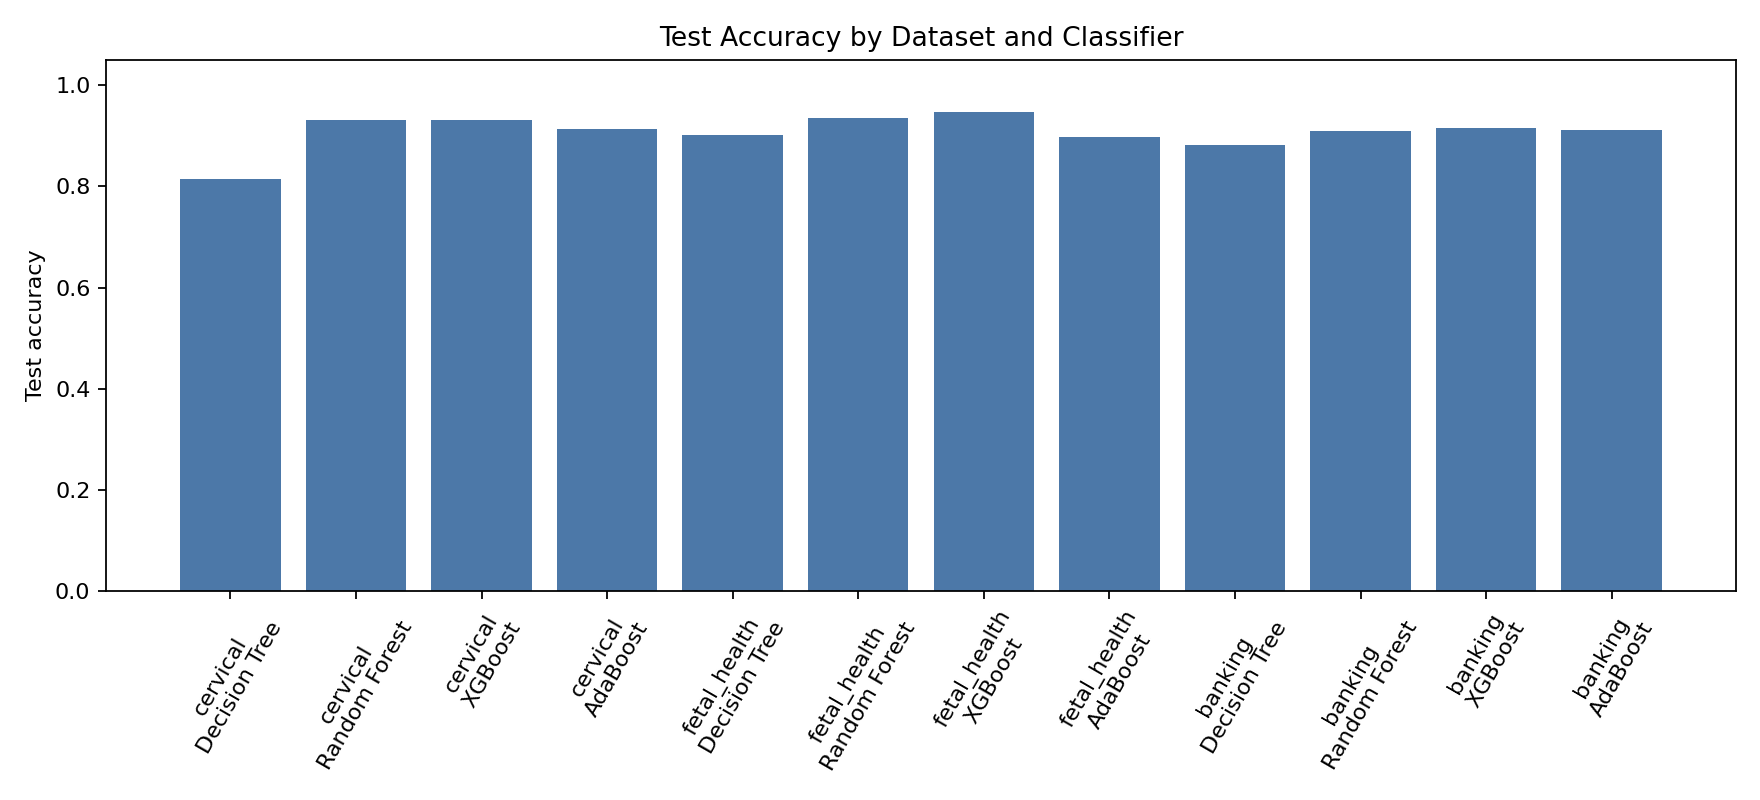
\includegraphics[width=\textwidth]{images/test_accuracy_summary.png}\caption{Test accuracy summary.}\end{figure}
\begin{figure}[H]\centering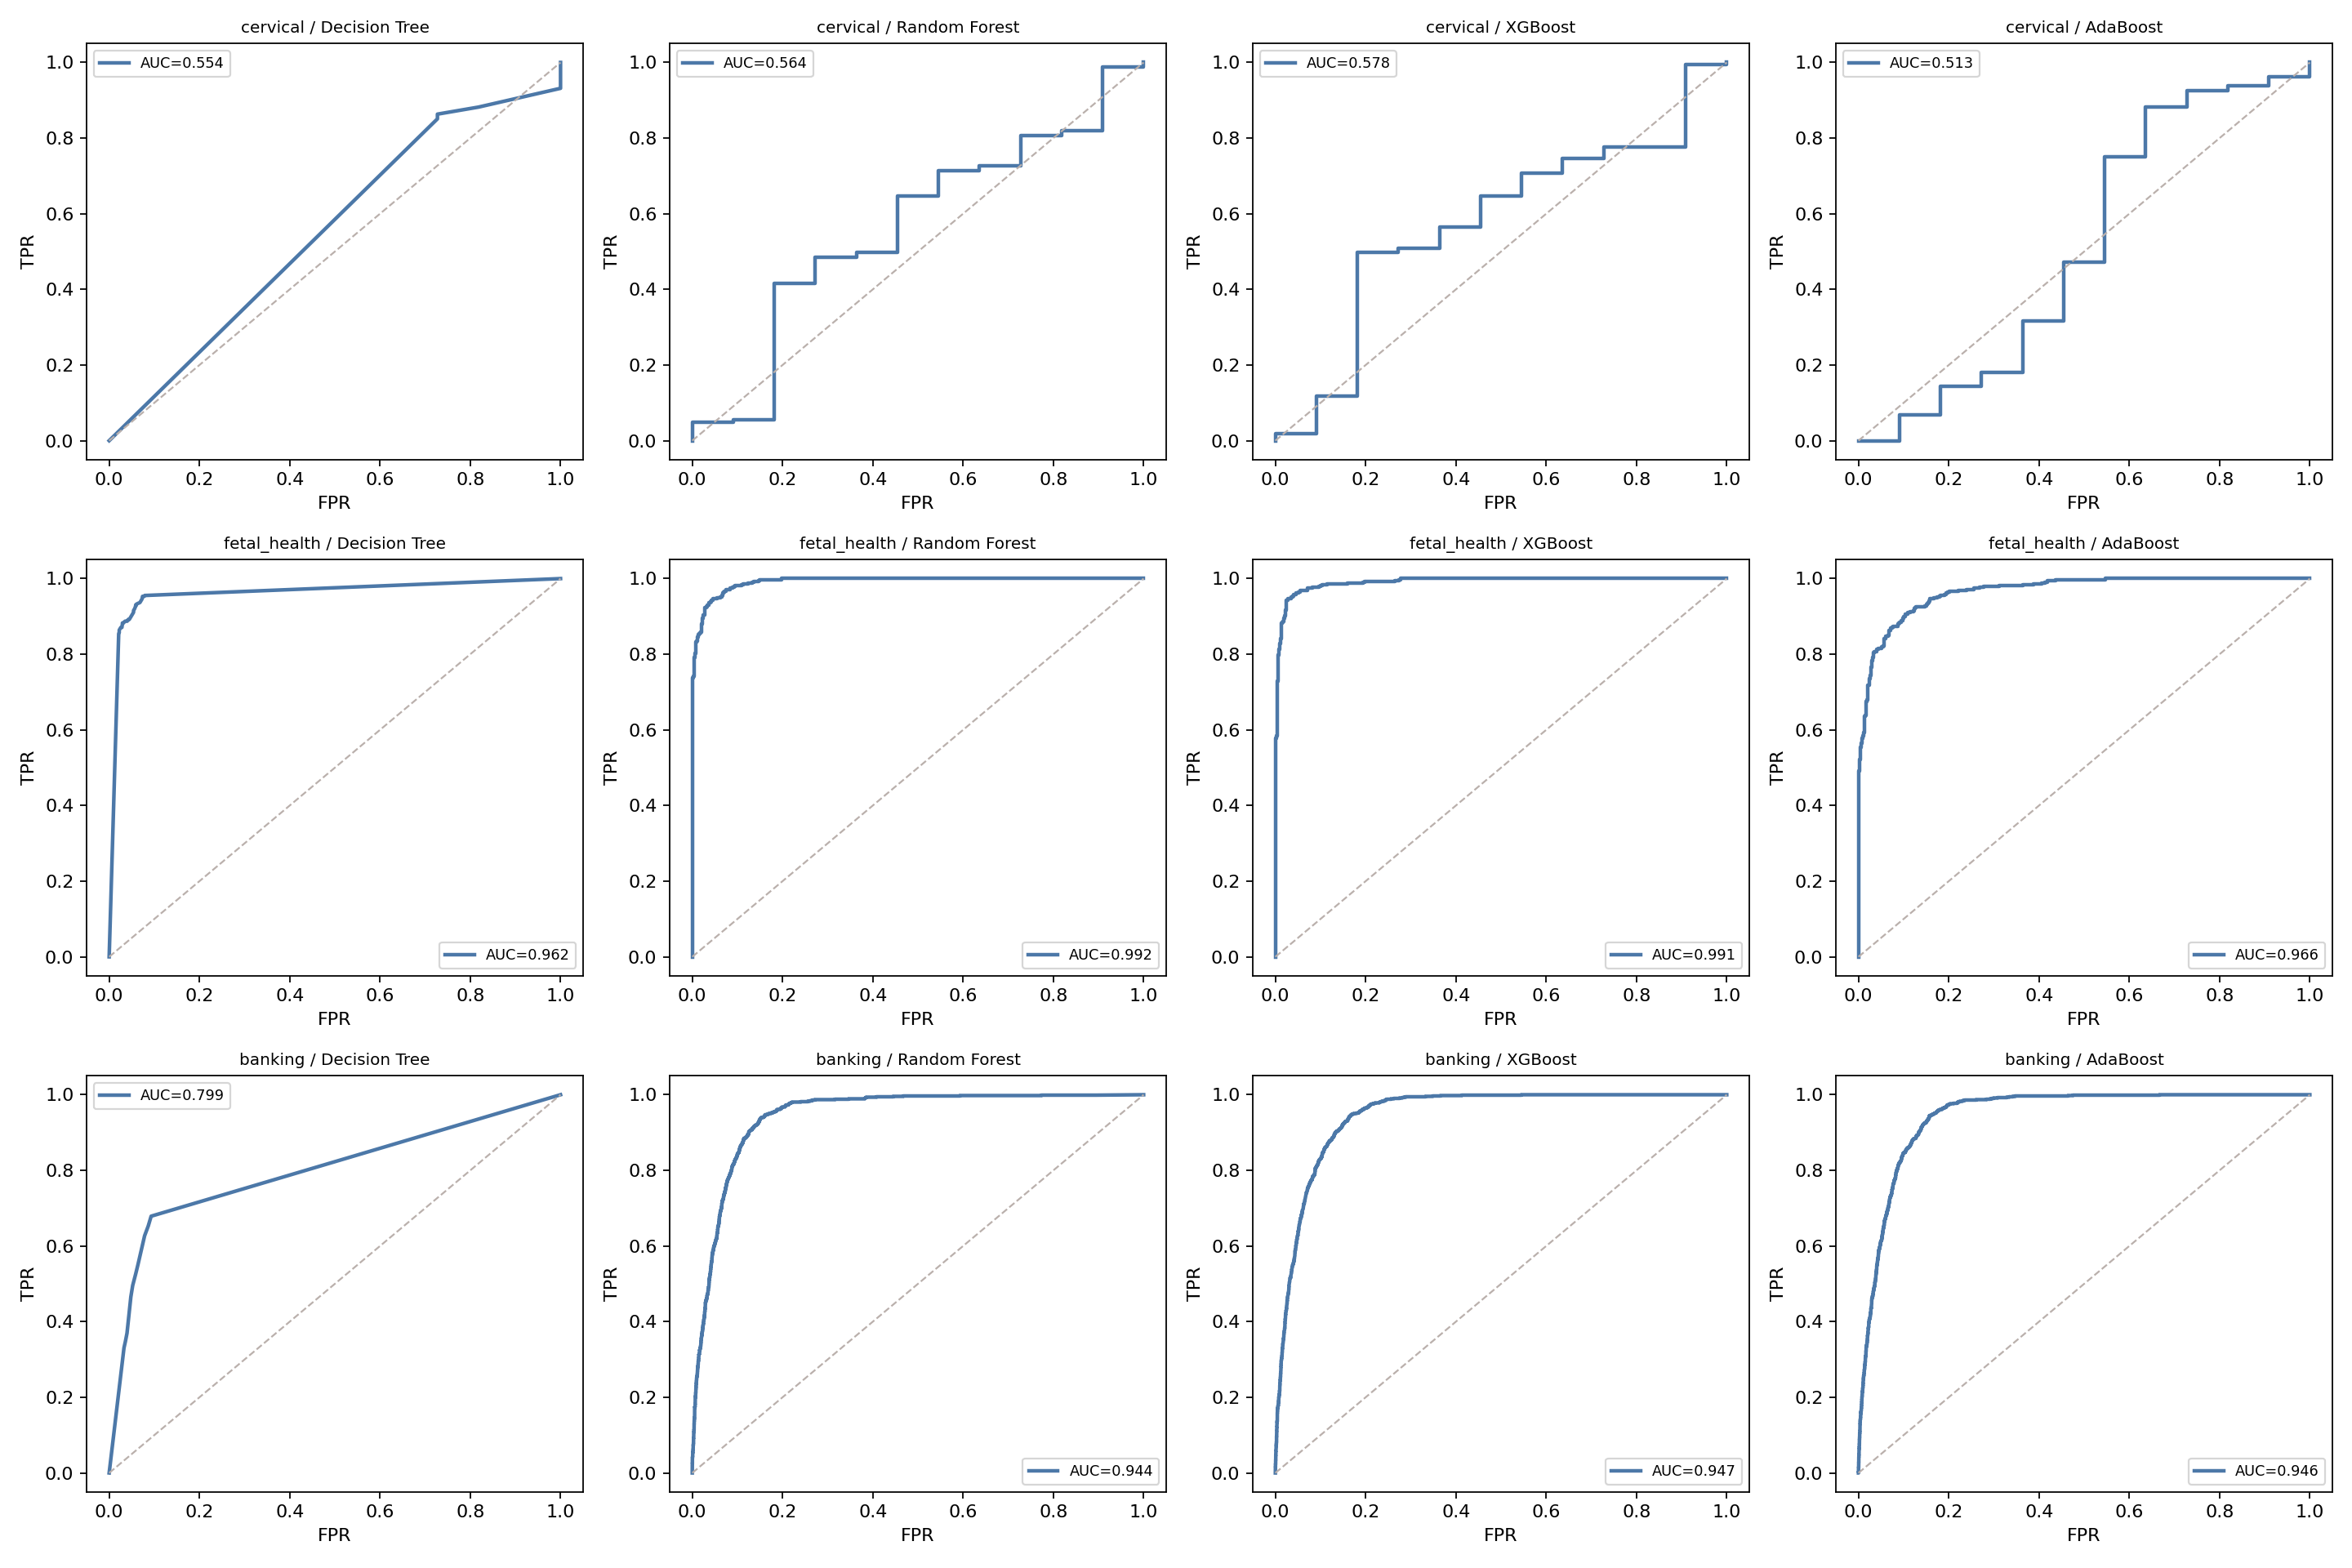
\includegraphics[width=\textwidth]{images/roc_curves.png}\caption{ROC curves.}\end{figure}
\begin{figure}[H]\centering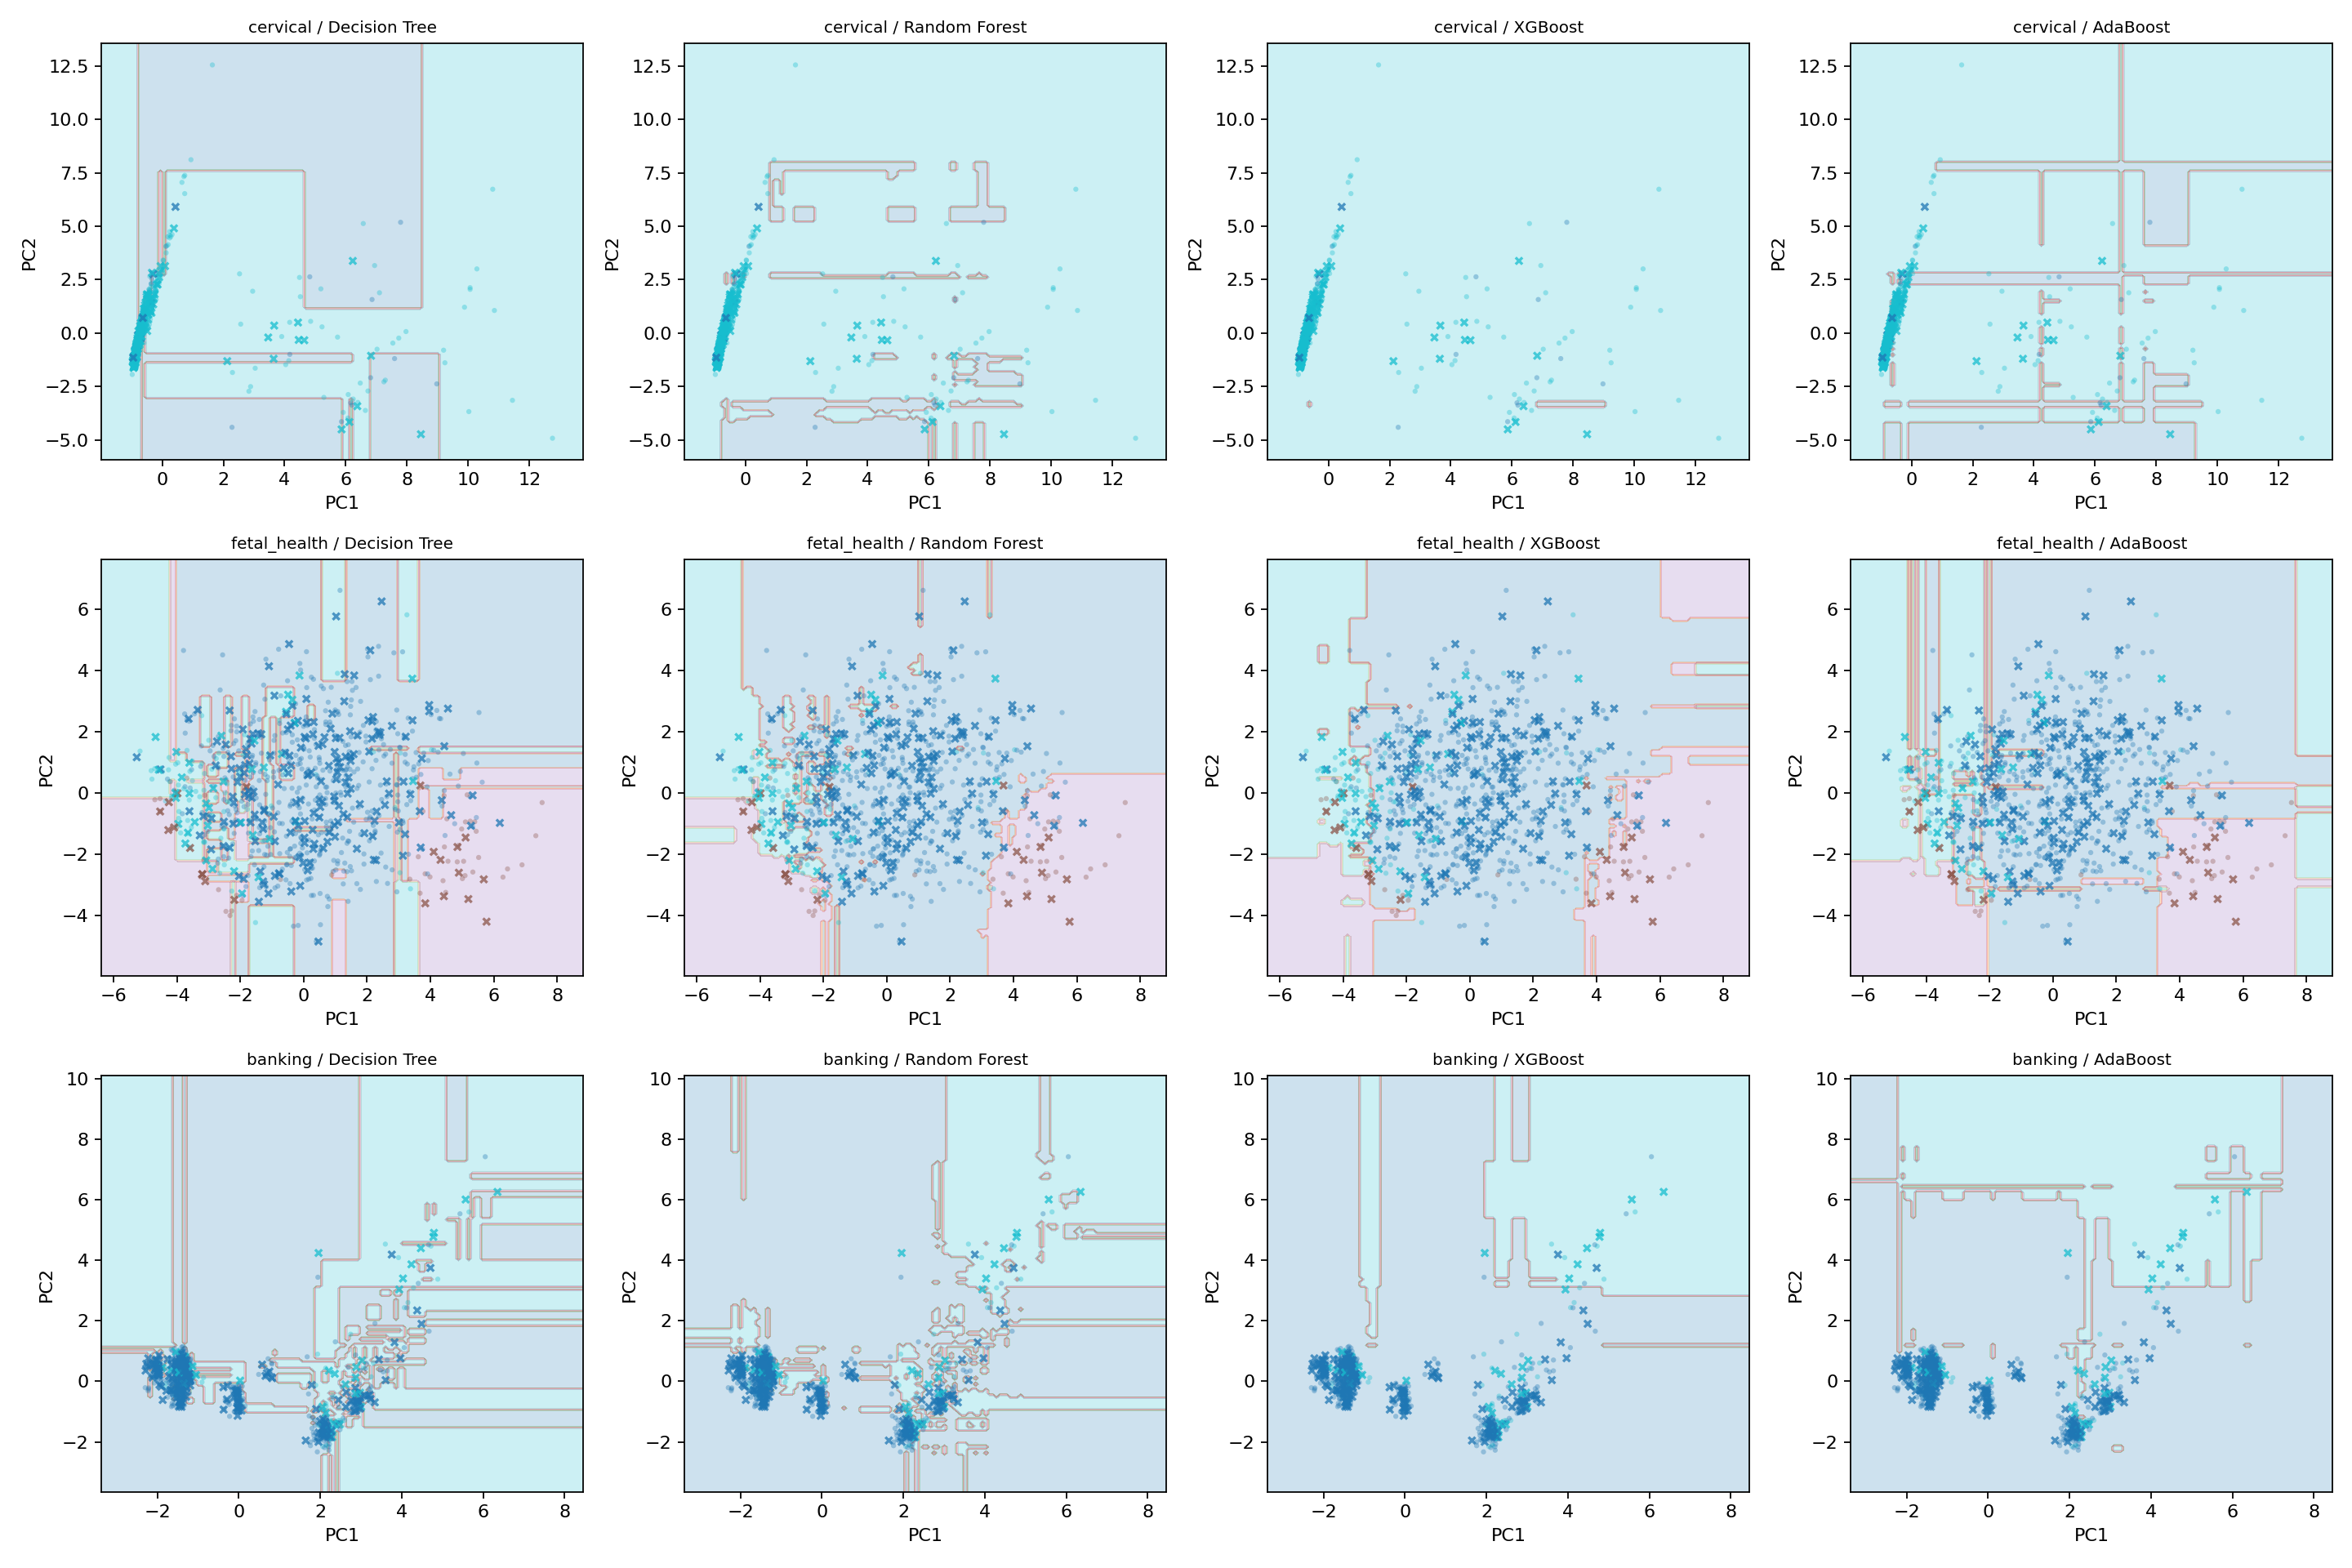
\includegraphics[width=\textwidth]{images/decision_boundaries.png}\caption{PCA decision-boundary visualizations.}\end{figure}
\end{document}